\chapter{Concreto de ultra alto desempenho ({CUAD})}

%\section{Introdução}

Sempre buscou-se o desenvolvimento de um concreto cada vez mais resistente e mais fácil de se trabalhar. Inicialmente, essas duas características se rivalizam, pois, a relação água/aglomerante influencia tanto a trabalhabilidade do concreto como sua resistência. Uma maior quantidade de água melhora a trabalhabilidade do concreto, mas aumenta sua porosidade e diminui sua resistência e durabilidade \cite{Guerra}. Por outro lado, se a quantidade de água for muito pequena, o concreto terá uma baixa trabalhabilidade, dificultando o trabalho dos operários.

\nomenclature[S]{MPa}{Megapascal}

Na década de 1930, Eugène Freyssinet demonstrou que, a aplicação de pressão no concreto fresco ainda na forma, aumentava sua resistência mecânica, devido à diminuição ou até mesmo eliminação dos vazios. Nos anos 60, apenas com a aplicação deste princípio (com elevada pressão) e cura térmica, foram alcançados valores de resistência de 650 MPa \apud[p.~8]{Richard_e_Cheyrezi}{Vanderlei}.

%.

%O desenvolvimento de superplastificantes (para diminuir a relação água/aglomerante), aditivos, pigmentos e fibras para concreto, assim como o uso de técnicas inovadoras de execução podem, teoricamente, fazer com que o concreto possa atender qualquer solicitação de projeto, tendo como limitante apenas o custo da execução.

Pode-se dizer que CUAD é uma classe de concretos com resistência e durabilidade superiores ao CAD (concreto de alto desempenho). 

Segundo \citeonline[p.~5]{Resplendino}, as primeiras pesquisas sobre a tecnologia do CUAD começaram nos anos 70, com o pesquisador Bache, na Dinamarca. Suas pesquisas resultaram no desenvolvimento do CRC (\textit{Compact Reinforced Composite}, em português, CCR - Compósito Compacto Reforçado). Na Europa o CRC é muito utilizado na composição de pré-fabricados, porém eles são reforçados por armaduras convencionais, calculadas de modo que não se leva em consideração a participação mecânica das fibras \cite[p.~6]{Resplendino}. Segundo \apudonline[p. ~30]{Aitcin}{Tutikian}, nos anos 1972-1973, Brunanauer desenvolveu um compósito capaz de resistir uma solicitação de compressão de até 200 MPa, o qual foi patenteado sob o nome de DSP (\textit{Densified with Small Particles} ou DPP - Densificado de Partículas Pequenas), baseado no conceito de compactação da matriz granulométrica. Posteriormente, Birchall et al. desenvolveram um concreto de ultra alto desempenho a partir de uma abordagem diferenciada, denominado de MDF (\textit{Macro Deffect Free} ou LMD - Livre de Macros Defeitos) \apud{Aitcin}{Tutikian}. O MDF incorpora o conceito de pasta polimérica, garantindo uma resistência a tração na flexão de 150 MPa ou mais, especialmente quando se utiliza cimento aluminoso. Desse modo, as principais linhas de pesquisa da atualidade se dividem em dois ramos: uma pesquisa a utilização de materiais finíssimos na composição do concreto e a outra, a utilização de pastas poliméricas na composição do concreto \cite[p.~8]{Vanderlei}.

\nomenclature[A]{CRC}{\textit{Compact Reinforced Composite}}
\nomenclature[A]{CCR}{Compósito Compacto Reforçado}
\nomenclature[A]{DSP}{\textit{Densified with Small Particles}}
\nomenclature[A]{DPP}{Densificado de Partículas Pequenas}
\nomenclature[A]{MDF}{\textit{Macro Deffect Free}}
\nomenclature[A]{LMD}{Livre de Macros Defeitos}

Diversos compósitos de base cimentícia possuem alta resistência e superior durabilidade, os quais pode-se dizer que se enquadram na categoria de concreto de ultra alto desempenho (CUAD). Além das variedades citadas acima, por \citeonline{Russel_e_Graybeal} e outras de desenvolvimento mais recente, tem-se:

\begin{alineas}[label=\textbullet]
  %\item CRC - \textit{compact reinforced composite} (CCR - compósito compacto reforçado);
  \item FRHPC - fiber-reinforced high-performance concrete (CADRF - concreto de alto desempenho reforçado com fibras);
  \item HPFRCC - high-performance fiber reinforced cement composite (CCADRF - compósito cimentício de alto desempenho reforçado com fibras);
  \item MSFRC - multi-scale fiber-reinforced concrete (CMSRF - concreto multiescalável reforçado com fibras);
  \item RPC - reactive powder concrete (CPR - concreto de pós reativos);
  \item SFCBC - steel fibrous cement-based composite (CCFA - compósito cimentício fibroso de aço)
  \item UHPFRCC - ultra-high performance fiber-reinforced cementitious composite (CCUADRF - compósito cimentício de ultra alto desempenho reforçado com fibras);
  \item UHPFRC - ultra-high performance fiber-reinforced concrete (CUADRF - concreto de ultra alto desempenho reforçado com fibras);
  \item UHSC - ultra-high strength concrete (CUAR - concreto de ultra alta resistência);
  \item Compósito cimentício de ultra alta resistência;
  \item Compósito cimentício de ultra resistência reforçado com fibras.
  \item UHPGC - ultra-high performance glass concrete (CVUAD - concreto de vidro de ultra alto desempenho) \footciteref{Soliman};
  \item GUHPC - geopolymer composite ultra high performance concrete (CGCUAD - compósito geopolimérico de concreto de ultra alto desempenho)\footciteref{Gong}.
\end{alineas}

\nomenclature[A]{FRHPC}{\textit{Fiber-reinforced high-performance concrete}}
\nomenclature[A]{CADRF}{Concreto de alto desempenho reforçado com fibras}
\nomenclature[A]{HPFRCC}{\textit{High-performance fiber reinforced cement composite}}
\nomenclature[A]{CCADRF}{Compósito cimentício de alto desempenho reforçado com fibras}
\nomenclature[A]{MSFRC}{\textit{Multi-scale fiber-reinforced concrete}}
\nomenclature[A]{CMSRF}{Concreto multiescalável reforçado com fibras}
\nomenclature[A]{RPC}{\textit{Reactive powder concrete}}
\nomenclature[A]{CPR}{Concreto de pós reativos}
\nomenclature[A]{SFCBC}{\textit{Steel fibrous cement-based composite}}
\nomenclature[A]{CCFA}{Compósito cimentício fibroso de aço}
\nomenclature[A]{UHPFRCC}{\textit{Ultra-high performance fiber-reinforced cementitious composite}}
\nomenclature[A]{CCUADRF}{Compósito cimentício de ultra alto desempenho reforçado com fibras}
\nomenclature[A]{UHPFRC}{\textit{Ultra-high performance fiber-reinforced concrete}}
\nomenclature[A]{CUADRF}{Concreto de ultra alto desempenho reforçado com fibras}
\nomenclature[A]{UHSC}{\textit{Ultra-high strength concrete}}
\nomenclature[A]{CUAR}{Concreto de ultra alta resistência}
\nomenclature[A]{UHPGC}{\textit{Ultra-high performance glass concrete}}
\nomenclature[A]{CVUAD}{Concreto de vidro de ultra alto desempenho}
\nomenclature[A]{GUHPC}{\textit{Geopolymer composite ultra high performance concrete}}
\nomenclature[A]{CGCUAD}{Compósito geopolimérico de concreto de ultra alto desempenho}

Historicamente, pode-se observar uma relação muito próxima entre a tecnologia existente e os materiais disponíveis para construção e a arquitetura das construções. Ainda que o CUAD seja chamado de “concreto”, trata-se de um material completamente novo, exigindo um novo olhar sobre como ele deve ser utilizado nas construções. Não faz nenhum sentido utilizar um material com desempenho tão elevado do mesmo modo que utilizamos o concreto convencional. A popularidade de um material é diretamente afetada pelo seu custo. Assim como a produção de aço foi revolucionada pela Bessemer and Open Hearth Steel na década de 1850, produzindo aço em grande escala a preços acessíveis, fazendo com que as pessoas passassem a utilizá-lo nas construções, o CUAD também precisa passar por um processo similar, de modo que essa tecnologia possa ser trazida a aplicações populares \cite[p.~9]{Tang}.

Neste trabalho, utiliza-se a definição genérica concreto de ultra alto desempenho (CUAD), salvo quando houver necessidade de especificar uma variedade.

\section{Definição do CUAD}

A \citeonline[p.~7, tradução nossa]{AFGC} define CUAD da seguinte maneira:

\begin{citacao}
"Concreto de ultra alto desempenho reforçado com fibras"~se refere a materiais com matriz cimentícia e características de resistência à compressão que excedem 150 MPa, possivelmente chegando a 250 MPa, e contendo fibras de aço para atingir comportamento dúctil sob tensão e, se possível, dispensar o uso de armadura passiva (não protendida). Também pode conter polímeros.
\end{citacao}

\nomenclature{CAD}{Concreto de alto desempenho}

A \citeonline[p.~7, tradução nossa]{AFGC} ainda destaca que o CUAD se diferencia do concreto de alto de desempenho (CAD) conforme as seguintes características:

\begin{citacao}
\textbullet~~O CUAD possui uma resistência a compressão maior que 150 MPa, enquanto o CAD varia entre 35 MPa e 100 MPa; \\ 
\textbullet~~O CUAD usa fibras, assegurando que o material não seja quebradiço e modificando os requisitos convencionais para reforço com armadura passiva/ativa. O CAD normalmente não possui fibras; \\
\textbullet~~O CUAD usa muito aglomerante de modo a reduzir drasticamente o uso de água e possui seleção especial de agregados.
\end{citacao}

Desse modo, pode-se definir que CUAD é um compósito composto de aglomerante, agregado miúdo, fibras (metálicas, naturais ou sintéticas) que, ao contrário do concreto convencional, é capaz de suportar grandes cargas de compressão e possui comportamento dúctil, devido às fibras adicionadas ao compósito. Caracteriza-se também pela alta quantidade de aglomerante, baixa relação água/aglomerante (o que garante um material de alta densidade) baixa porosidade (conforme mostrado na \autoref{porosidade}), microestrutura extremamente cerrada e cura térmica a elevadas temperaturas. Desse modo, este material possui uma elevada durabilidade, possui baixa permeabilidade para cloridos (composto químico extremamente corrosivo para concreto), grande resistência a congelamento-descongelamento e grande resistência a ataques de ácidos e sulfatos \cite[p.~7-11]{Resplendino}.

Segundo o \citeonline{CBI}, pode-se dizer, resumidamente, que o CUAD é composto de (\autoref{componentes}): 

\begin{alineas}[label=\textbullet]
  \item cimento;
  \item fíler (quartzo, pó de cinza, escória);
  \item areia;
  \item água;
  \item superplastificante;
  \item fibras (metálicas ou poliméricas).
\end{alineas}

E caracteriza-se por:

\begin{alineas}[label=\textbullet]
  \item baixa relação água/aglomerante;
  \item alta dosagem de superplastificante;
  \item auto adensamento;
  \item microestrutura densa (\autoref{empacotamento});
  \item cura térmica.
\end{alineas}

É importante notar que o cimento não é o único aglomerante que pode ser utilizado para fazer o CUAD. Pesquisas recentes mostram que alternativas como geopolímeros e pó de vidro podem substituí-lo na mistura dos materiais, os quais podem ser até mais sustentáveis e baratos que o cimento \cite{Goldoni} \cite{Soliman}.

\begin{figure}[htb]
	\caption{\label{porosidade}Porosidade do CUAD em relação ao concreto convencional.}
	\begin{center}
	    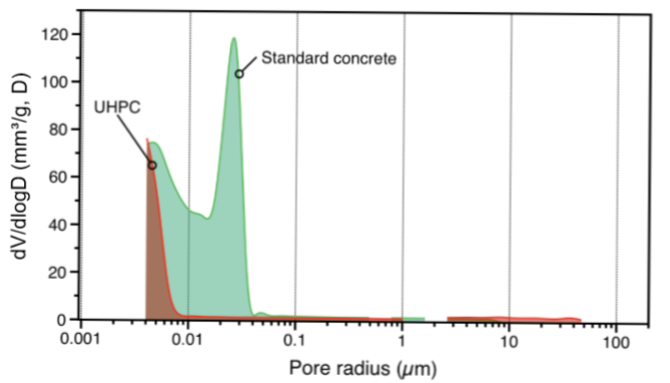
\includegraphics[max width=\textwidth]{porosidade.png}
	\end{center}
	\fonte{\citeonline{CBI}}
\end{figure}

\begin{figure}[htb]
	\caption{\label{componentes}Materiais que compõem o CUAD.}
	\begin{center}
	    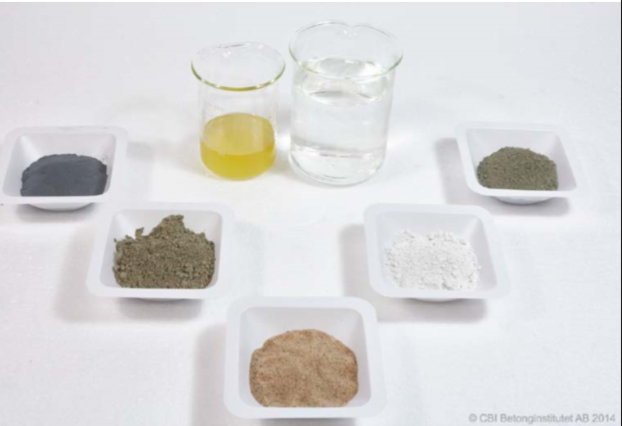
\includegraphics[max width=\textwidth]{componentes.png}
	\end{center}
	\fonte{\citeonline{CBI}}
\end{figure}

\begin{figure}[htb]
	\caption{\label{empacotamento}Comparação entre a microestrutura dos agregados no concreto padrão x CUAD.}
	\begin{center}
	    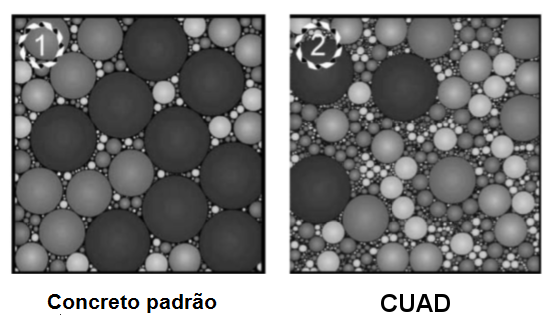
\includegraphics[max width=\textwidth]{empacotamento.png}
	\end{center}
	\fonte{\citeonline{CBI}}
\end{figure}

Tipicamente, o CUAD resiste a solicitações de compressão de 200 MPa e à ruptura dúctil de 10 a 15 MPa. Ainda é capaz de suportar deformação e carregamentos de flexão e tensão mesmo após a fissuração inicial do concreto, devido à dissipação de energia do material ser maior devido à sua microestrutura densa \cite[p.~1]{Gunes}.

\section{CUAD do tipo CPR (concreto de pós reativos)}

Existe muitas variedades de CUAD disponíveis no mercado, mas segundo \citeonline[p.~1312-1313]{Tutikian}, o CPR (concreto de pós reativos) é o CUAD que possui a maior dedicação dos centros de pesquisa. É sobre essa variedade de CUAD que este trabalho se concentra.

\citeonline[p.~1313]{Tutikian} afirma que a “ideia básica desse novo tipo de concreto foi eliminar os inconvenientes dos agregados graúdos [...] como as possíveis oclusões ou vazios internos, eliminação da zona de transição e aumento da superfície do esqueleto granular”. O seguinte excerto explica melhor suas características:

\begin{citacao}
Pelo efeito da maior superfície específica, a distribuição das cargas incidentes sobre os grãos é mais homogênea, diminuindo a concentração de tensões em eventual falha da microestrutura, assim, aumentando a resistência última do material. Sabe-se que, quanto menor a dimensão dos grãos, maior é a superfície específica, maior a reatividade química e ligações secundárias pelas forças de van der Waals (ligações de superfície) e mais elevada é a homogeneidade do material. Dessa forma, os grãos de agregados finos não ficam em contato um com os outros, evitando as tensões de contato e possíveis falhas nesses locais \cite[p.~1312]{Tutikian}.
\end{citacao}

\apudonline[p.~1314]{Aitcin}{Tutikian} resume o conceito do CPR em três princípios básicos:

\begin{citacao}
\textbullet~Aumento da homogeneidade do material pela eliminação das partículas grossas, limitação da areia para prevenir que entrem em contato entre si na pasta endurecida, melhoria nas propriedades mecânicas da pasta de cimento hidratada e eliminação da zona de transição nas interfaces pasta/agregados;\\
\textbullet~Aumento da compacidade pela otimização das dimensões dos grãos dos pós da mistura e, quando possível, pela compressão exercida durante o endurecimento;\\
\textbullet~Refinamento da microestrutura da pasta hidratada por tratamento de calor.
\end{citacao}

\citeonline{Vanderlei_e_Giongo} definem os princípios para obtenção do CPR da seguinte forma:

\begin{alineas}[label=\textbullet]
  \item eliminação dos agregados graúdos para aumentar a homegeinidade;
  \item compressão do material durante o preparo (antes e durante a concretagem, diminuindo a incorporação de ar, removendo o excesso de água e compensando a retração química) e/ou otimização da distribuição granulométrica dos agregados miúdos de modo a aumentar a densidade do material;
  \item cura térmica para fortalecer a microestrutura;
  \item uso de fibras ou tubos metálicos preenchidos com CPR para aumentar a ductilidade;
\end{alineas}

Do ponto de vista da granulometria dos agregados que compõem o CPR (diâmetro máximo de 0,2 mm), ele deveria ser considerado uma argamassa, mas convencionou-se chamá-lo de concreto devido ao desempenho exibido pelo material \cite[p.~1313]{Tutikian}.

\citeonline{Vanderlei_e_Giongo} demonstram que a indústria brasileira já produz os materiais necessários para obtenção do CPR. Assim como \citeonline{Tutikian},  recomendam o uso de cimento CPV ARI. A dosagem de CPR proposta por \citeonline{Vanderlei_e_Giongo} é mostrada na \autoref{dosagem-cpr}.

\begin{table}[htb]
\IBGEtab{%
  \caption{Dosagem para concretos de pós reativos.}
  \label{dosagem-cpr}
}{%
  \begin{tabulary}{\linewidth}{CCC}
  \toprule
   Material                 & Relação (em massa) & Consumo $kg/m^3$ \\
  \midrule \midrule
   Cimento                  & 1                  & 874 \\ \midrule 
   Areia                    & 1,101              & 962 \\ \midrule 
   Pó de quartzo            & 0,235              & 205 \\ \midrule 
   Sílica ativa             & 0,246              & 214 \\ \midrule 
   Superplastificante (3\%) & 0,030              & 26  \\ \midrule 
   Água (a/c = 0,18)        & 0,180              & 157 \\
  \bottomrule
\end{tabulary}%
}{%
  \fonte{\citeonline[p.~119]{Vanderlei_e_Giongo}.}%
  \nota{Recomenda-se o uso de água de amassamento de baixa temperatura, pré cura térmica de 2 dias e cura térmica de 24 horas a uma temperatura de 80\textsuperscript{\degree} C.}
  %\nota[Anotações]{Uma anotação adicional, que pode ser seguida de várias outras.}
  }
\end{table}

É importante notar que a dosagem \citeonline{Vanderlei_e_Giongo} é condizente com a realidade brasileira, portanto difere da utilizada por outros estudos internacionais, em virtude da diferença geográfica.

A adição de fibras é o fator determinante na resistência à tração na flexão do CPR, que passam a influenciar este fator em uma taxa a partir de 1\% \cite[p.~138]{Vanderlei_e_Giongo}. A \autoref{taxa-fibras} mostra a influência da taxa de fibras na resistência à tração na flexão do CPR observada nos corpos de prova moldados pelos autores.

\begin{figure}[htb]
	\caption{\label{taxa-fibras}Influência da taxa de fibras na resistência à tração na flexão do CPR.}
	\begin{center}
	    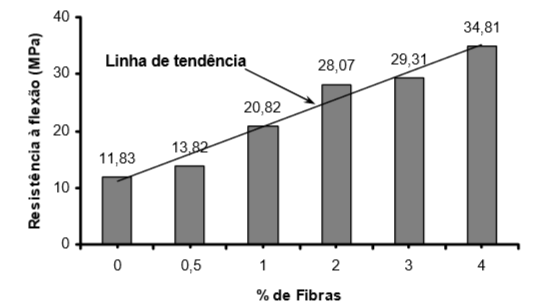
\includegraphics[max width=\textwidth]{taxa-fibras.png}
	\end{center}
	\fonte{\citeonline[p.~138]{Vanderlei_e_Giongo}}
\end{figure}

Ainda não existe uma consolidação de como deve ser feito o estudo de dosagem do CPR. \citeonline[p.~42]{Vanderlei} e \citeonline[p.~32]{Christ} informam que métodos matemáticos de empacotamento de partículas têm bastante êxito nessa tarefa.

\subsection{Componentes da mistura}
A utilização do concreto sempre tem como objetivo a obtenção de uma mistura com resistencia, trabalhabilidade e desempenho, sendo assim o desenvolvimento tecnologico do concreto passou a focar na otimização dos componentes que constituem a mistura, no modo de preparação e analise o objetivo final de sua utilização. Essa escala de analise faz com que o conceito de concreto fosse modificado em relaçaõ ao seu significado mais tradicional, passando a pensar no concreto como uma elemento de estético e não mais como um aglutinador de elementos.

As pesquisas realizadas desempenharam um papel de extrema importancia no conceito da construção, possibilitando a descoberta de concretos que pudessem desempenhar funções especificas de acordo com a necessidade exigida pela situção. Assim partiu-se de um concreto convencional, passando pelo concreto armado e chegando ao CAUD, que é definido pela ACI (1998) apud Tutikian (2011) como: um concreto que atenda uma combinação especial entre desempenho e requesitos de uniformidade que não pode ser atingida rotineiramente com uso de componentes concvencionais e praticas normais de mistura, lançamento e cura.

O principal diferencial que distingue o CAUD dos outros tipos de concreto está atrelado à justificativa de sua utilização, já que sua composição é basicamente a mesma em relação ao concreto convencional e aproveitando das mesmas materias-primas. Podendo essa justificativa estar relacionada ao meio em que o concreto estará exposto, a resistencia requerida, ao desemprenho ao longo do tempo ou até esbeltez da area ou perfil. E para que esse desempenho seja asseguradao necessitou-se de uma acompanhamento especifíco em todos os componentes da mistura como: fator agua/aglomerante; granulometria dos agregados miudos e graudos; adição de aditivos, processo de cura e adensamento.

Destrinchando os aspectos que influenciam diretamente o desenvolvimento do CAUD vimos que o fator agua/aglomerante esta intrinsicamente relacionado a resistencia mecanica, que seus agregados devem ser escolhidos de maneira cuidadosa para que a porosidade da mistura não seja afetada, a escolha dos aditivos é feita de maneira específica para cada finalidade, assim como os processos de manuseio, cura a e adensamento. Em essência, esses são os pontos básicos para uma mistura de CAUD, que sempre tem como objetivo primario uma compacidade maior entre seus componentes, para que sempre tenha como resultado uma pasta compctada com baixo teor de porosidade e microestrutura cerrada.

Para que esse resultado seja obtido necessita-se que: tenha uma diminuição do fator agua/aglomerante, relação agua/m³ e do ar aprisionado na massa, atraves de aditivos ou superplastificantes; escolha adequada dos agregados miúdos em relação a granulometria para uma maior compacidade, passando a ser mais fino que o proprio cimento em alguns casos; utilização de agragados graudos com menor diametro, isso faz com que essa parte do processo ganhe uma importancia elevada pois essa fase do concreto tende a ser a parte mais fragil da mistura, podendo comprometer a resistencia final; reforços das ligações quimicas entre as particulos atraves de adiçoes minerais que provocam o refinamento dos poros e grãos, como a silica ativa, metacaulim ou as cinzas de arroz, tambem conhecidas como superpozolanas. As consequencias diretas dessas ações resultam em uma microestrutura com poros de menor tamanho, resistencia a passagem de fluidos e maior capacidade de fixação de agentes dissolvidos. O resultado final dessa gama de processos nos leva a um aumento da compacidade, alta resistencia mecânica, elevação da durabilidade e de seu desempenho ao longo de sua vida util.

Assim evidencia-se que alem da busca por melhores materiais baseados na sua fabricação, temos que direcionar nossa atenção para as fases de agragados, zona de transição e pasta, entendenso que as fases possuem seu inicio na seleção de agregados e os processos subsequentes tem o começo inteiramente ligado ao termino do processo anterior. 
 
->Adicionar Tutikian 36.8.1,2,3,4 e 36.9


\section{Sustentabilidade e custo-benefício}

Segundo \citeonline[p.~797, tradução e grifo nosso]{Racky}

\begin{citacao}
O custo-benefício sempre foi a maior exigência dos engenheiros civis nos processos de projeto, planejamento e construção. A partir da década de 1990, o princípio da sustentabilidade foi incluído, de modo a atender às demandas sociais, fazendo com que o custo-benefício deixasse de se preocupar apenas com fatores puramente de otimização econômica e passasse a integrar fatores sociais e ecológicos. \textbf{Custo-benefício e sustentabilidade não são mutuamente excludentes}. Pelo contrário, custo-benefício é um componente integral do conceito de sustentabilidade.
\end{citacao}

\citeonline{Racky} demonstra que o consumo energético (fabricação, transporte, etc.) do ciclo produtivo do CUAD, se comparado de maneira bruta, é maior que o do concreto convencional, culminando na liberação de gases poluentes e potenciais danos ambientais. Mas isso não leva em consideração que o CUAD abre novas possibilidades de projeto ao viabilizar a construção de estruturas mais leves esbeltas, além de aumentar o espaço útil destas construções. Levando isso em consideração, tem-se resultados animadores, onde ocorre uma economia energética entre 58\% e 74\%. É importante salientar as limitações do estudo, que faz essa comparação em relação a pilares de concreto convencional e pilares feitos com CUAD.

\citeonline[p.~801]{Racky} ainda aponta outros benefícios:

\begin{alineas}[label=\textbullet]
  \item diminuição do uso de concreto;
  \item quantidades menores armadura;
  \item menor área de formas.
\end{alineas}

O que, consequentemente, leva à uma otimização do tempo de construção, ou seja, diminuição do custo e dos prazos de entrega da obra.

\citeonline{Tutikian} afirma que estruturas feitas com o CUAD do tipo CPR são capazes de atingir dimensões e valores de resistência semelhantes ao do aço, porém com menor custo, maior esbeltez e durabilidade. A \autoref{cuad-secao} mostra as quatro seções com a mesma capacidade portante, onde é possível ver que as dimensões e o peso especifíco da estrutura feita com CPR é bem próximo do aço.

\begin{figure}[htb]
	\caption{\label{cuad-secao}Comparação entre seções de diferentes materiais com a mesma capacidade portante.}
	\begin{center}
	    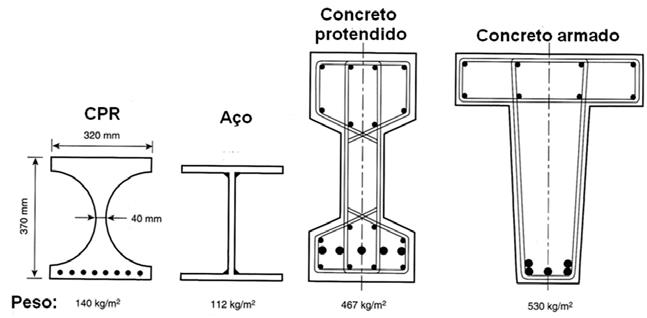
\includegraphics[max width=\textwidth]{cuad-secao.png}
	\end{center}
	\fonte{\apudonline[p.~1320]{Walraven}{Tutikian}}
\end{figure}

\citeonline[p.~803]{Racky} ainda aponta uma economia a longo prazo, que inclui a manutenção, reparo e demolição da construção.

\section{CUAD no mundo}

Muitas construções já foram feitas com CUAD em diversos países. O Canadá, pioneiro na utilização do material ainda em 1997, possui mais de 26 construções, entre pontes, passarelas e viadutos \cite{Russel_e_Graybeal}. A \autoref{construcoes-cuad} lista algumas construções feitas em CUAD ao redor do mundo.

\begin{table}[htb]
\IBGEtab{%
  \caption{Exemplos de aplicações de CUAD ao redor do mundo.}
  \label{construcoes-cuad}
}{%
  \begin{tabulary}{\linewidth}{CCCCCC}
  \toprule
   Estruturas/aplicações & Local & Ano & Resistência à compressão (MPa) & Resistência à flexão (MPa) \\
  \midrule \midrule

   Passarela Sherbrooke	           & Sherbrooke, Canadá      & 1997 & 200 &	40	\\ \midrule 
   Silo de clínquer Joppa	       & Illinois, EUA           & 2001 & 220 &	50	\\ \midrule 
   Passarela Seonyu	               & Seul, Coréia do Sul     & 2002 & 180 &	32	\\ \midrule 
   Passarela Sakata Mirai	       & Sakata, Japão           & 2002 & 238 &	40	\\ \midrule 
   Pedágio no Millau Viaduct	   & Rodovia A75, França     & 2002 & 165 &	30	\\ \midrule 
   Ponte da angra Sheperds	       & Sydney, Austrália       & 2005 & 180 &	-	\\ \midrule
   Painéis resistentes a explosão  & Melbourne, Australia    & 2005 & 160 & 30  \\ \midrule 
   Passarela Papatoetoe	           & Auckland, Nova Zelândia & 2006 & 160 &	30	\\ \midrule 
   Ponte Glenmore/Legsby	       & Calgary, Canadá         & 2007 & -	  &	-	\\ \midrule 
   Ponte Gaertnerplatz	           & Kassel, Alemanha        & 2007 & 150 &	35	\\ \midrule 
   Ponte Jakway Park               & Iowa, EUA               & 2008 & 150 &	-	\\ \midrule 
   Fundações de turbina eólica	   & Dinamarca               & 2008 & 210 &	24	\\ \midrule
   Lajes do Aeroporto de Haneda	   & Tóquio, Japão           & 2010 & 210 & 45	\\ \midrule 
   Ponte Whiteman Creek	           & Brantford, Canadá       & 2011 & 140 & 30	\\ \midrule
   Canos de esgoto                 & Germany                 & 2012 & 151 & –   \\ \midrule
   Colunas do tipo "spun"          & Germany                 & 2012 & 179 & –   \\ \midrule
   Passarela de treliças de CUAD   & Espanha                 & 2012 & 150 & –	\\
  \bottomrule
\end{tabulary}%
}{%
  \fonte{\citeonline[p.~273.]{Abbas}.}%
  %\nota{Esta é uma nota, que diz que os dados são baseados na regressão linear.}
  %\nota[Anotações]{Uma anotação adicional, que pode ser seguida de várias outras.}
  }
\end{table}

Segundo \citeonline{Russel_e_Graybeal}, a Alemanha iniciou, em 2005, um programa com 34 projetos de pesquisa divididos entre 20 instituições, de modo desenvolver a base necessária para os estudos técnicos sobre CUAD e torná-lo ``um produto confiável, disponível rotineiramente, economicamente acessível e regularmente aplicado''.

Desde a publicação das recomendações para usar CUAD em estruturas na França\footciteref{AFGC}, em 2002, muitas pontes já foram executadas. O Japão\footciteref{JSCE} também publicou um conjunto similar de recomendações em 2006 \cite{Russel_e_Graybeal}.

A Coréia do Sul está pesquisando o uso de CUAD em pontes estaiadas, mostrando que esse material ganha cada vez mais atenção internacional \cite{Russel_e_Graybeal}.

%\section{{CUAD} disponível no mercado} -> [Capítulo removido]

\citeonline{Resplendino} lista os principais concretos de ultra alto desempenho disponíveis no mercado:

\begin{alineas}[label=\textbullet]
  \item Ductal\textsuperscript{\textregistered}, marca comercial do CPR, comercializado pela Lafarge (França);
  \item BSI/CERACEM\textsuperscript{\textregistered}, desenvolvido pelo grupo EIFFAGE SIKA (França);
  \item BCV\textsuperscript{\textregistered}, desenvolvido pelo grupo Vicat (França);
  \item CEMTECmultiscale\textsuperscript{\textregistered}, desenvolvido pela LCPC (França);
  \item Materiais laboratoriais desenvolvidos pela EDF (Électricité de France, companhia elétrica francesa), do CERIB (Centre d’Études et de Recherches de l’Industrie du Béton, em português: Centro de Estudos e Pesquisas da Indústria do Concreto) (França);
  \item CRC, sob a marca comercial Densit\textsuperscript{\textregistered}, desenvolvido pela Aalborg Portland Cement (Dinamarca);
\end{alineas}

Ainda existe o COR-TUF\textsuperscript{\textregistered} \footciteref{Durst}, desenvolvido pelo \textit{US Army Corps of Engineers Engineer Research and Development Center} (em português, Centro de Pesquisa e Desenvolvimento de Engenharia do Corpo de Engenheiros do Exército dos Estados Unidos), o qual ainda procura parceiros comerciais para licenciar e comercializar o COR-TUF\textsuperscript{\textregistered}. Outro CUAD que pode ser encontrado no mercado é o DURA\textsuperscript{\textregistered} \footciteref{Dura}, produzido por uma empresa de mesmo nome, na Malásia.

\section{CUAD no Brasil}

No Brasil, já é possível encontrar o Ductal\textsuperscript{\textregistered} na fachada de dois edifícios na cidade de São Paulo: no edifício do Escritório de Representação do Ministério das Relações Exteriores (\autoref{fachada_ministerio_1} e \autoref{fachada_ministerio_2}) e na fachada da Japan House (\autoref{fachada_japan_house_1} e \autoref{fachada_japan_house_2}).

\begin{figure}[htb]
	\caption{\label{fachada_ministerio_1}Fachada executada com o CUAD Edifício do Escritório de Representação do Ministério das Relações Exteriores, na Rua da Consolação, São Paulo – SP.}
	\begin{center}
	    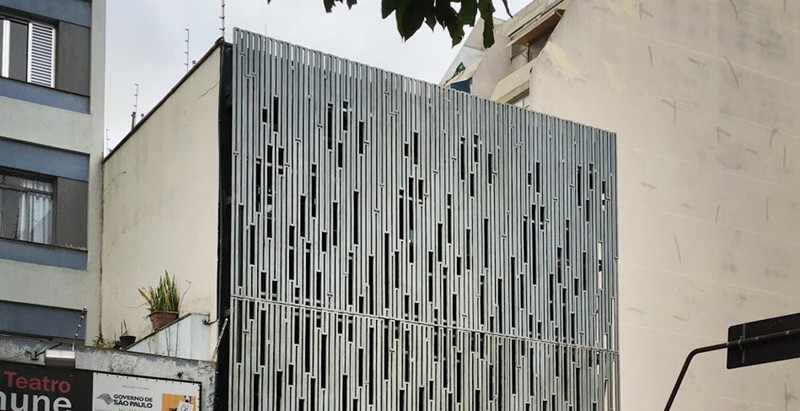
\includegraphics[max width=\textwidth]{fachada-ministerio-1.jpg}
	\end{center}
	\fonte{\citeonline{Stone}.}
\end{figure}

\begin{figure}[htb]
	\caption{\label{fachada_ministerio_2}Detalhe da fachada do mesmo edifício da \autoref{fachada_ministerio_1}.}
	\begin{center}
	    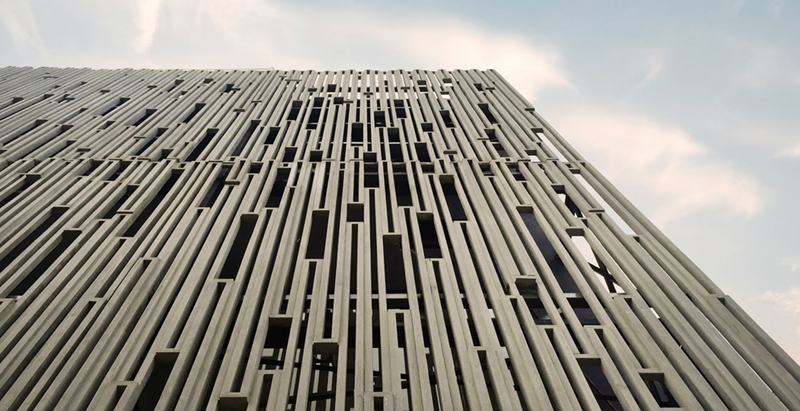
\includegraphics[max width=\textwidth]{fachada-ministerio-2.jpg}
	\end{center}
	\fonte{\citeonline{Stone}.}
\end{figure}

\begin{figure}[htb]
	\caption{\label{fachada_japan_house_1}Fachada executada com CUAD. Japan House, na Avenida Paulista, São Paulo - SP.}
	\begin{center}
	    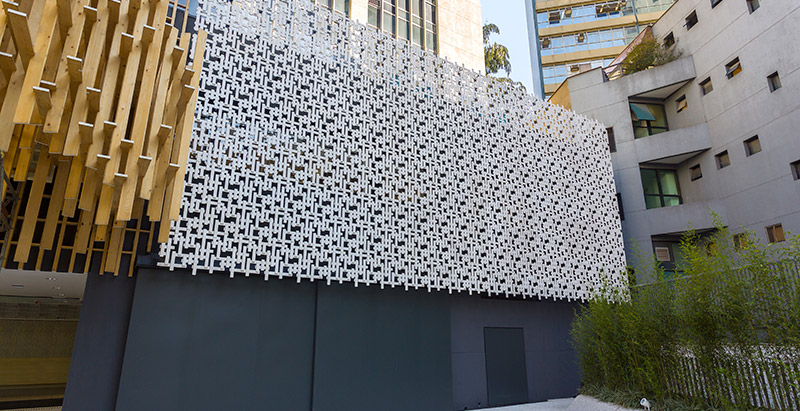
\includegraphics[max width=\textwidth]{fachada-japan-house-1.jpg}
	\end{center}
	\fonte{\citeonline{Stone}.}
\end{figure}

\begin{figure}[htb]
	\caption{\label{fachada_japan_house_2}Detalhe da mesma fachada da \autoref{fachada_japan_house_1}}
	\begin{center}
	    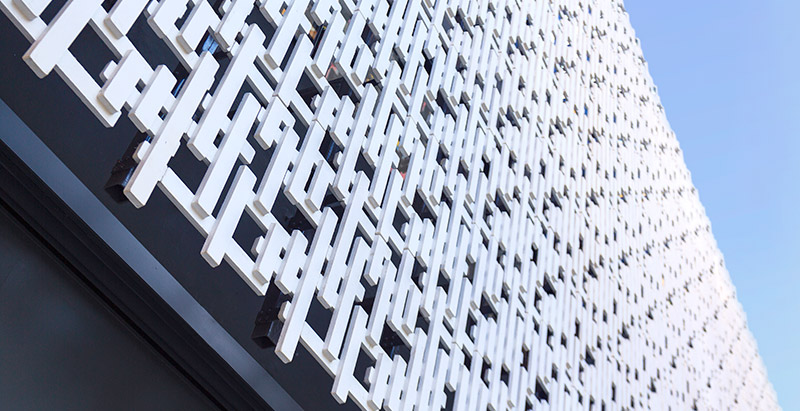
\includegraphics[max width=\textwidth]{fachada-japan-house-2.jpg}
	\end{center}
	\fonte{\citeonline{Stone}.}
\end{figure}

%\begin{figure}[htb]
%	\caption{\label{pulaski_skyway}Ponte Pulaski Skyway, New Jersey, EUA. Construída com CUAD.}
%	\begin{center}
%	    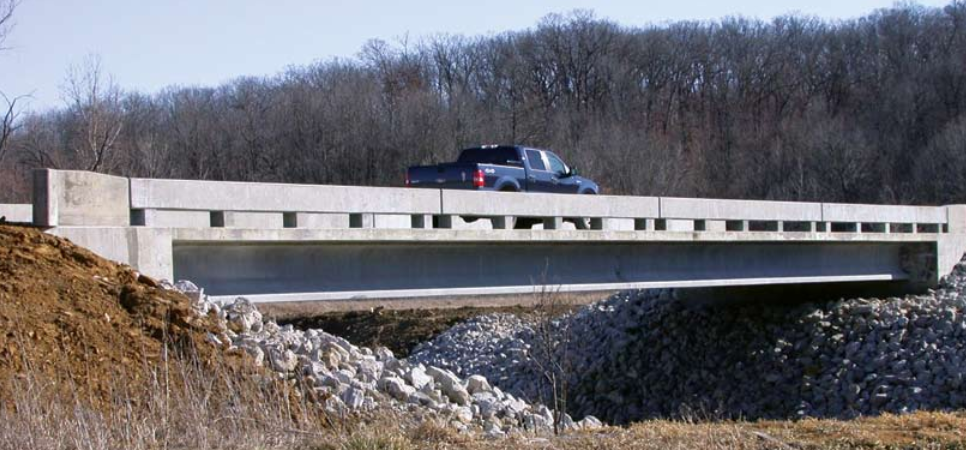
\includegraphics[max width=\textwidth]{ponte-pulaski-skyway.png}
%	\end{center}
%	\fonte{\citeonline{Stone}.}
%\end{figure}